\subsection{Multicore Models including Contention without Constraints}
\label{subsubsection: technical approach}

\begin{figure}[b!]
    \centering
    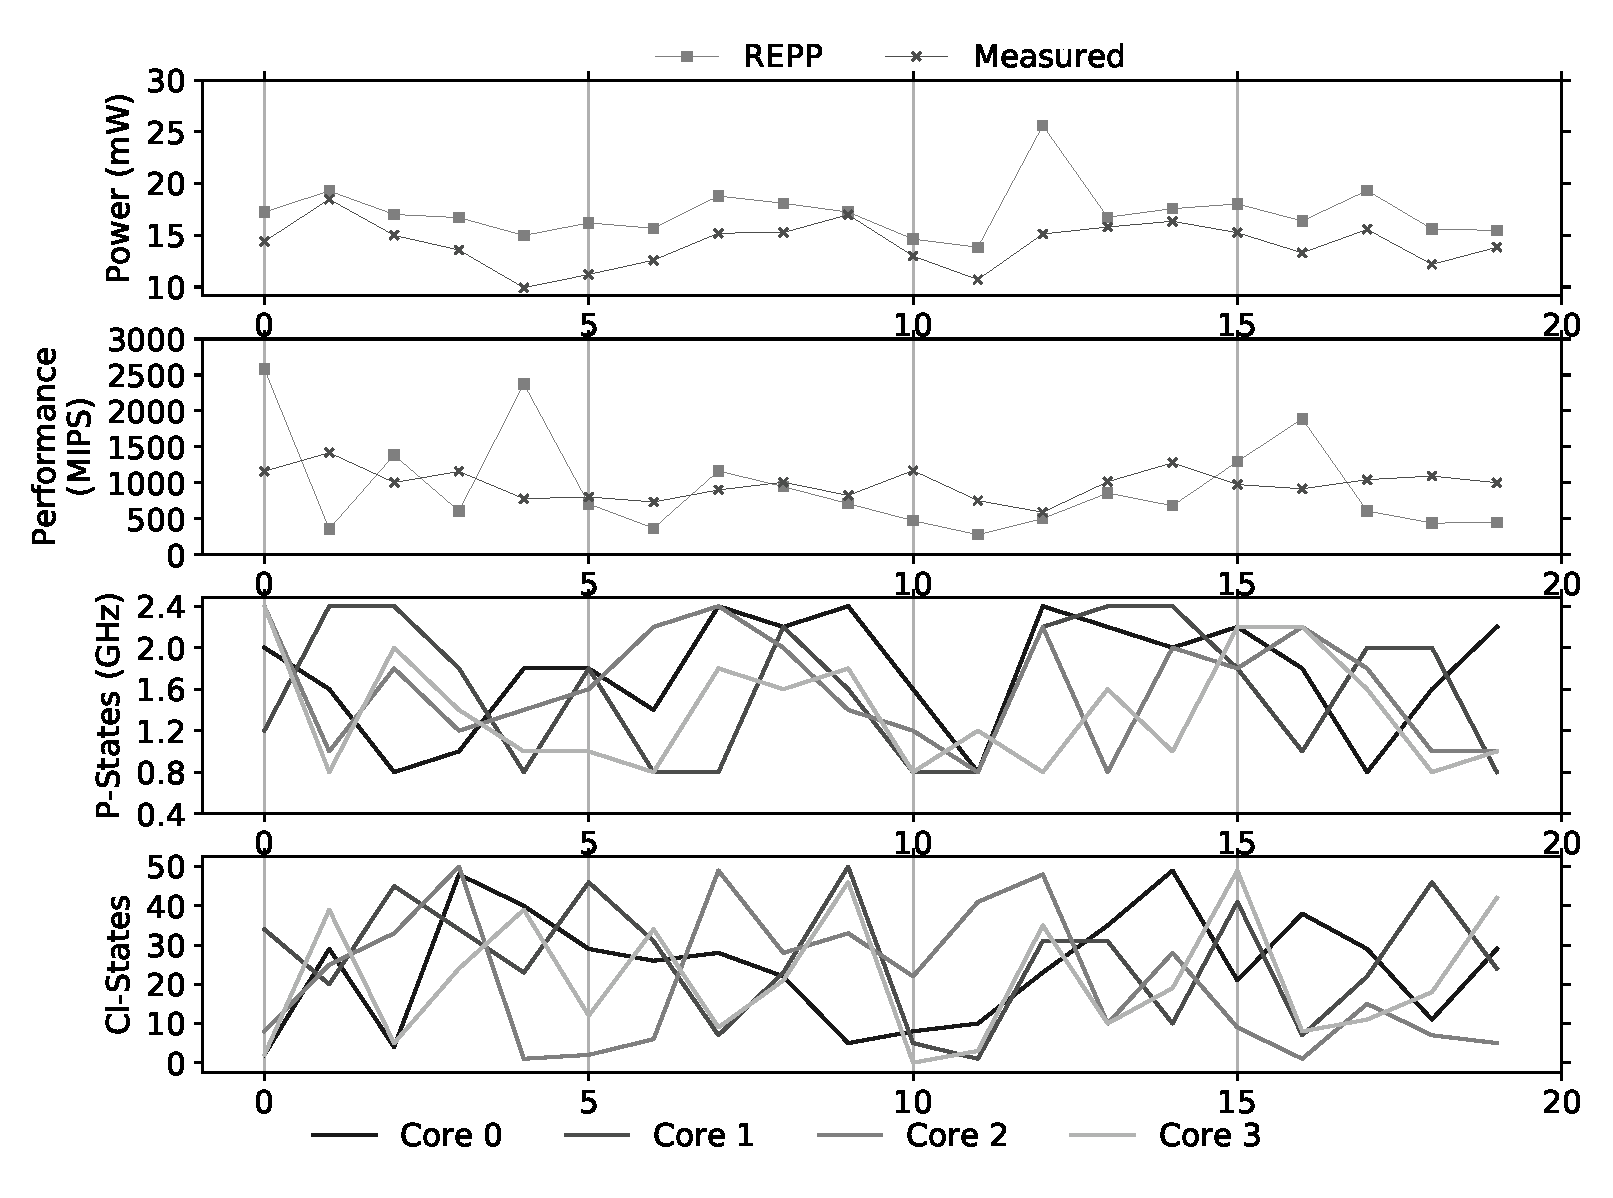
\includegraphics[width=\textwidth]{Chapter3/Figs/technical/SSSN-xal-xal-astar-blackscholes-new.eps}
    \caption[Power and performance prediction for workload SSSN]{\captitle{Power and performance prediction for workload SSSN.} Runtime power and performance prediction over time (in seconds) for workload SSSN. The legend at the top is for the first two graphs, and at the bottom is for the last two graphs.}
    %\caption{Runtime power and performance prediction over time (in seconds) for workload SSSN.}
    \label{fig: power realtimeSSSN}
    %./2016/repp-extention/perf-graphs.py script to regenerate plot
\end{figure}

Figure~\ref{fig: power realtimeSSSN} shows an example of the power and performance
prediction in runtime implemented on our system for the first 20 seconds of execution for
the workload, SSSN. Specifically the workload SSSN consists of benchmarks \emph{milc},
\emph{milc}, \emph{xalancbmk} and \emph{blackscholes}. From top-to-bottom, the first (and
second) graph represents the power (and performance) as measured using RAPL (and PMC) and
the prediction made using REPP. The third and fourth graphs show the random combination
of DVFS states and Cl-States generated for individual cores, respectively, for the first 20
seconds. We highlight two results. First, REPP does show the capability to adapt to
workloads consisting of multiple thread phases (SPEC CPU 2006 and PARSEC 3.0 benchmarks
have both memory and computational bound phases).  For instance, observe at second 12,
REPP makes a \SI{11}{\milli\watt} error in predicting power, this is because of the huge
changes in DVFS states and Cl-States. In this scenario, the DVFS states for core zero, one, two,
three change from \SI{0.8}{\giga\hertz} to \SI{2.4}{\giga\hertz}, \SI{0.8}{\giga\hertz} to
\SI{2.2}{\giga\hertz}, \SI{0.8}{\giga\hertz} to \SI{2.2}{\giga\hertz} and
\SI{1.2}{\giga\hertz} to \SI{0.8}{\giga\hertz} respectively and the Cl-States change from
10 to 23, 1 to 31, 41 to 48 and 3 to 35. Observe that these errors only occur with huge
changes in DVFS states and Cl-States in rapid intervals (for example, second four).  Ozlem
\etal~\citep{Bilgir_exploringthe} on the other hand, show that rapid changes in power or
performance are seldom required in data centre environments. Second, REPP can predict
power and performance per thread, which can not be accomplished using the in-built RAPL
register. In this particular workload, we make an error of \SI{9.4}{\percent}
(\SI{384}{\milli\joule}) and 15.2\% (1500 MIPS) when predicting power and performance over
300 seconds, respectively. 

\begin{figure}[t]
   \centering
    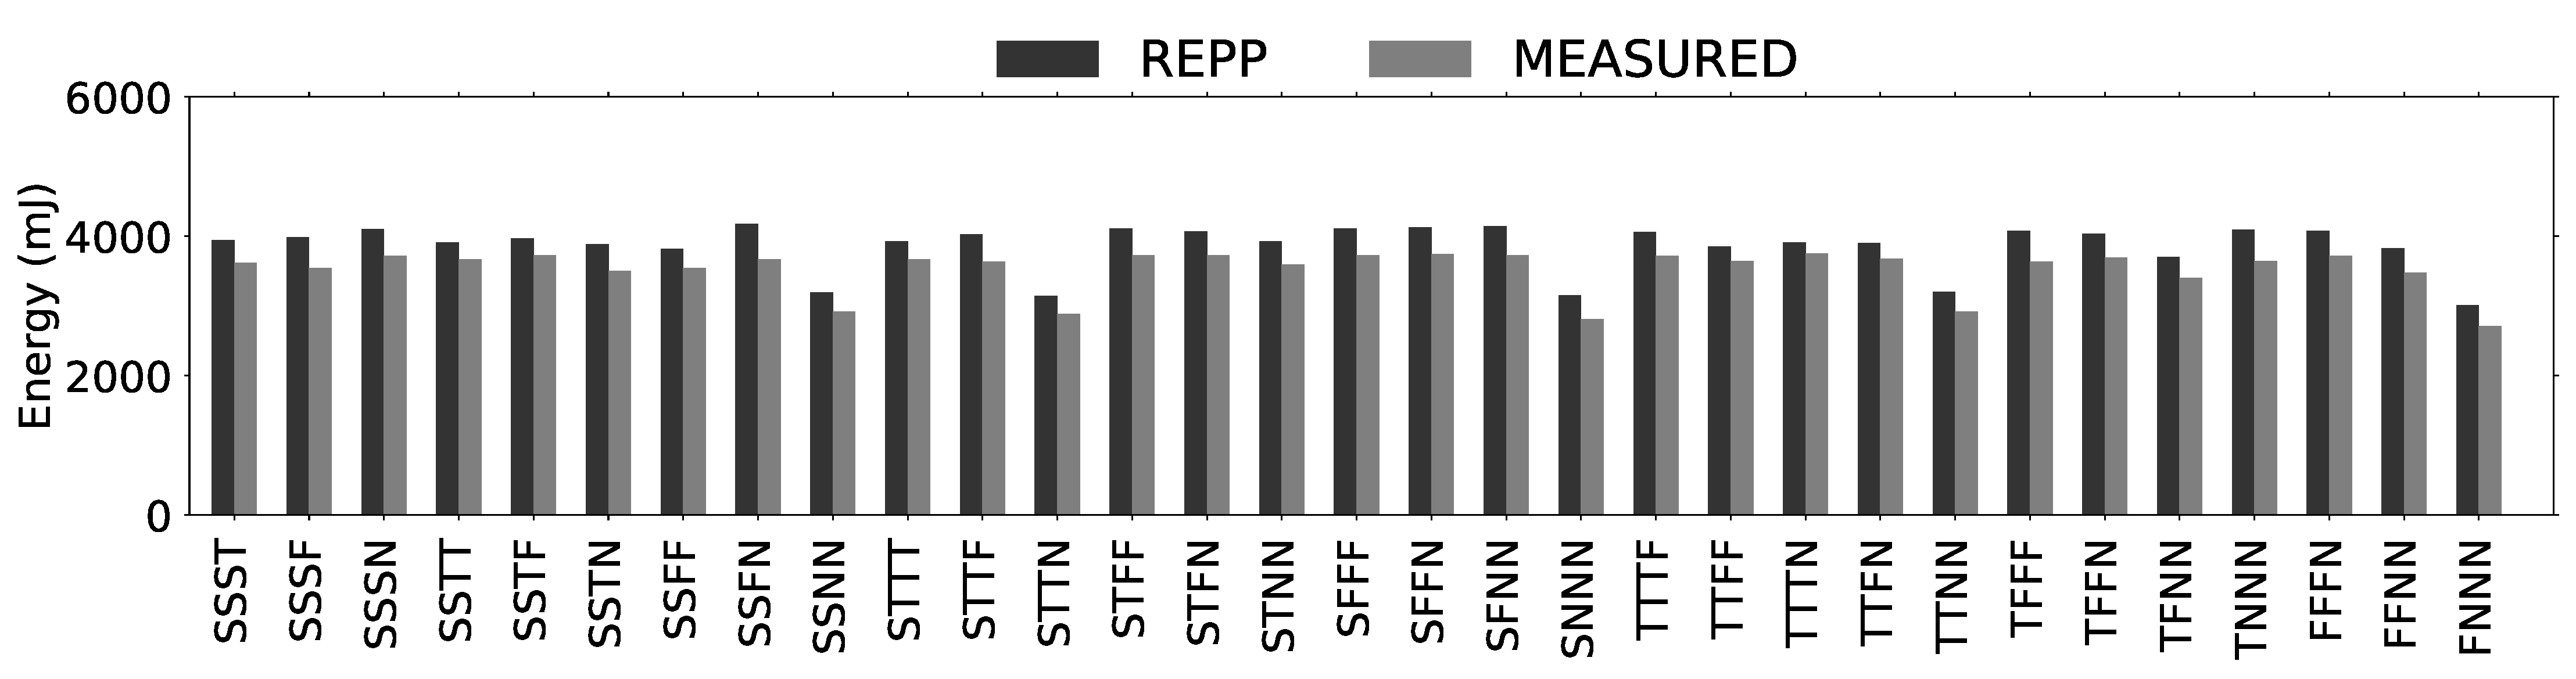
\includegraphics[width=\textwidth]{Chapter3/Figs/technical/power-paae.eps}
    \caption[Power prediction with multiple workloads without constraints]{\captitle{Power prediction for multiprogrammed workloads without constraints.} \textit{Energy consumed (\si{\milli\joule})} across all workloads on Intel processor. The $y$-axis is read as predicted (REPP) and measured (using RAPL).}
    \label{fig: power workloadswithout}
\end{figure}

Figure~\ref{fig: power workloadswithout} shows the energy consumption in
millijoules~(\SI{}{\milli\joule}) using our prediction technique, REPP and the power
measured using native RAPL register for all workloads over a period of 300 seconds when
switching across 1000 combinations of DVFS states and Cl-States. On average, workloads incur
an error in prediction of \SI{8.6}{\percent} or \SI{332.31}{\milli\joule}. Observe that
the maximum error we incur is \SI{12.1}{\percent} (\SI{507.36}{\milli\joule}) in workload
SSFN. 


\begin{figure}[t]
    \centering
    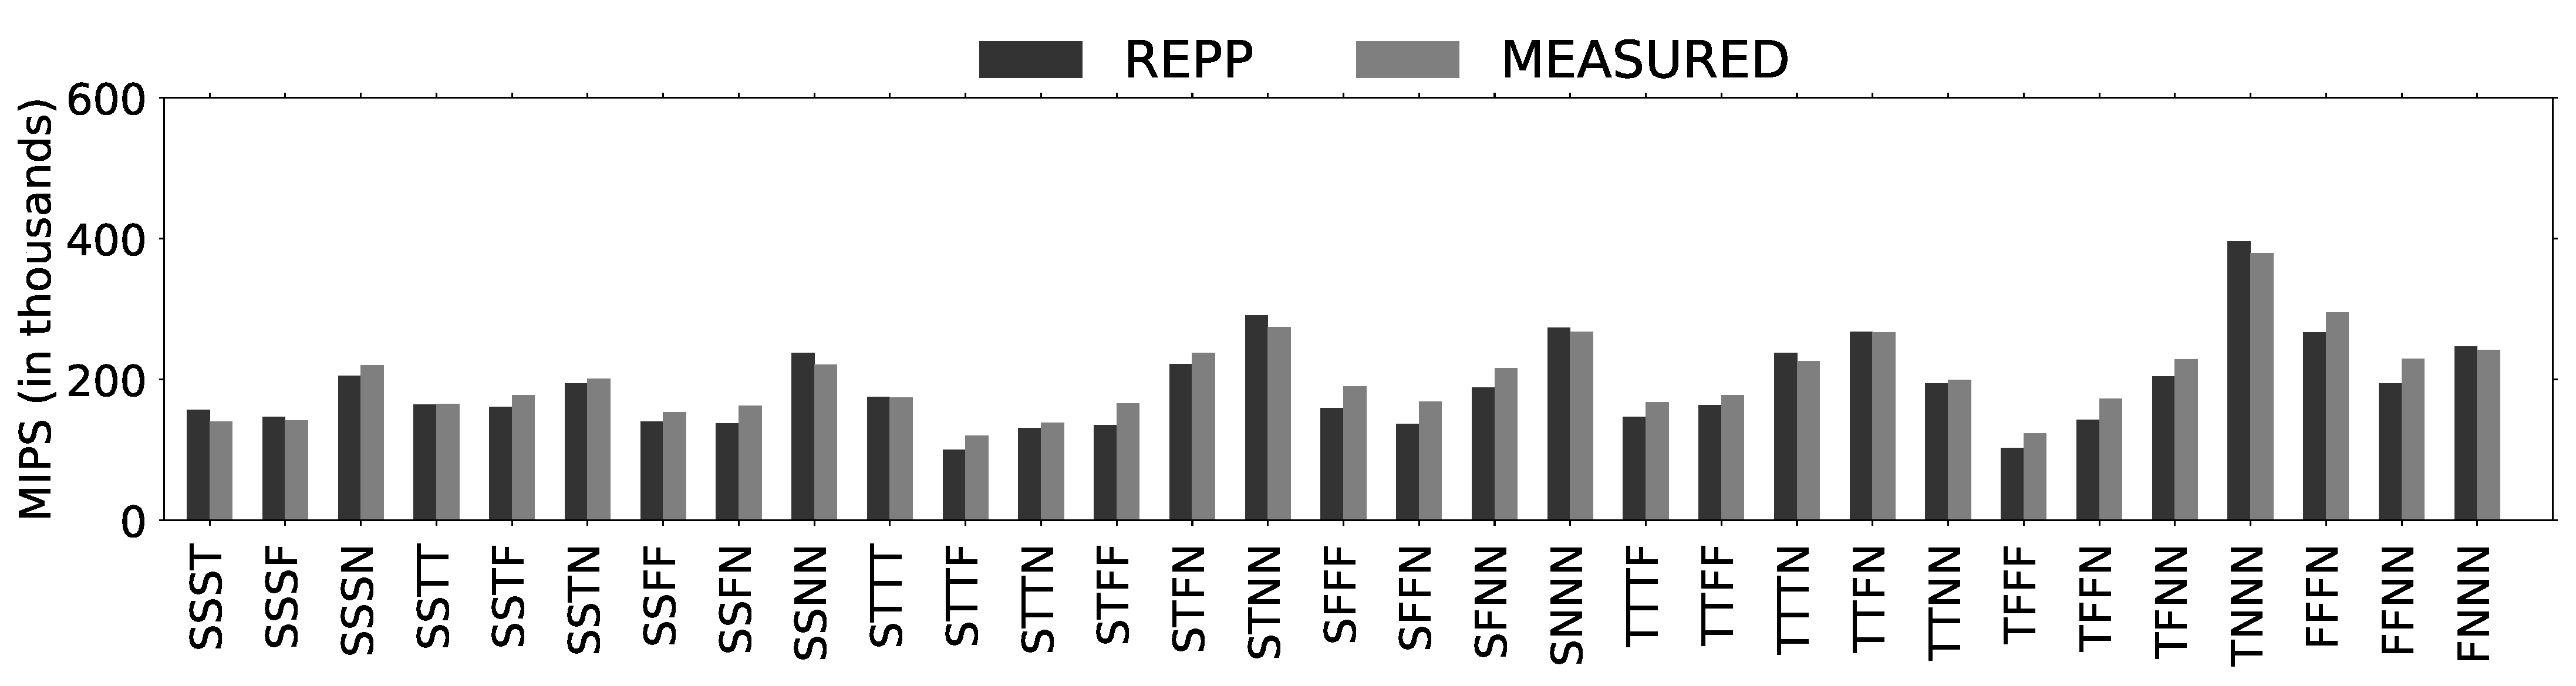
\includegraphics[width=\textwidth]{Chapter3/Figs/technical/perf-paae.eps}
    \caption[Performance prediction with multiple workloads without constraints.]{\captitle{Performance prediction for multiprogrammed workloads without constraints.} \textit{Total performance (in thousands)} across all workloads on Intel processor. The $y$-axis is read as predicted (REPP) and measured (using PMCs).}
    \label{fig: perf workloadswithout}
\end{figure}

Figure~\ref{fig: perf workloadswithout} shows the total performance (MIPS) in thousands
using our predicting technique (REPP), and the performance \texttt{measured} using PMCs
for all workloads over a period of 300 seconds when switching across 1000 combinations of
DVFS states and Cl-States. The average error we incur is \SI{8.8}{\percent} (over the 1000
combinations on all cores) and the maximum error is \SI{18.8}{\percent} in workload SFFN. 

\begin{table}[tb]
\centering
    \caption[Prediction error without constraints while disregarding certain benchmark categories]{\captitle{Performance and power prediction error without constraints while disregarding certain benchmark categories.} Error is shown in terms of PAAE.}
\scalebox{1}{    
\begin{tabular}{llccr} 
\toprule
    Label & Benchmark category & Power & Performance \\
\midrule
    N & Insensitive        & \SI{8.2}{\percent} & \SI{10.2}{\percent}    \\
    F & Cache-Friendly     & \SI{8.7}{\percent} & \SI{9.8}{\percent} \\
    T & Cache-Fitting      & \SI{9.6}{\percent} & \SI{9.9}{\percent} \\
    S & Thrashing          & \SI{8.2}{\percent} & \SI{7.5}{\percent} \\

\bottomrule
\end{tabular}
}
\label{tab: ignoringbenchmark}
\end{table}

Table~\ref{tab: ignoringbenchmark} shows the power and performance prediction error
without constraints for the remaining multiprogrammed workloads when disregarding certain
benchmark categories. It is observed that the power and prediction error for the remaining
benchmarks even after disregarding a subset of benchmarks is (approximately) same. 

Figure~\ref{fig: power workloadswithout} and~\ref{fig: perf workloadswithout} demonstrate that REPP
has been validated under multiple combinations of DVFS states and Cl-States across 35
multiprogrammed workloads. Moreover, each bar in the histogram represents a summary of the
workload execution, similar to Figure~\ref{fig: power realtimeSSSN}.
